\documentclass[12pt,a4paper]{article}

\usepackage[fleqn]{amsmath} % This package with the fleqn option aligns equations to the left
\setlength{\mathindent}{0pt} % Set indentation from the left margin

\usepackage{amssymb} % Required for math symbols
\usepackage{graphicx} % Required for inserting images
\usepackage{geometry}

\usepackage[backend=biber, style=authoryear, citestyle=authoryear]{biblatex}
\addbibresource{references.bib}

\geometry{a4paper, margin=1in}

{
\title{
    
\includegraphics[width=0.4\textwidth]{/Users/nicolasxx/documents/images/tsukuba-logo.png} \\
    \textbf{Practical Development for IoT and Embedded Systems} \\
    \vspace{3mm}    
    Report 2: Controlling LED on a Curcuit over the Network
}

\author{Mamanchuk Mykola, SID.202420671}
\date{\today}
}

\usepackage{listings}
\usepackage{color}

\definecolor{codegreen}{rgb}{0,0.6,0}
\definecolor{codegray}{rgb}{0.5,0.5,0.5}
\definecolor{codepurple}{rgb}{0.58,0,0.82}
\definecolor{backcolour}{rgb}{0.99,0.99,0.99}

\lstdefinestyle{mystyle}{
    backgroundcolor=\color{backcolour},   
    commentstyle=\color{codegreen},
    keywordstyle=\color{magenta},
    numberstyle=\tiny\color{codegray},
    stringstyle=\color{codepurple},
    basicstyle=\ttfamily\footnotesize,
    breakatwhitespace=false,         
    breaklines=true,                 
    captionpos=b,                    
    keepspaces=true,                 
    numbers=left,                    
    numbersep=5pt,                  
    showspaces=false,                
    showstringspaces=false,
    showtabs=false,                  
    tabsize=2
}
\lstset{style=mystyle}

\begin{document}

\maketitle

\section{Introduction}
This report describes the development and operation of an IoT application designed to control an LED via an Android tablet. This project utilizes a Raspberry Pi 4 Type B, various LEDs, and a MCIGICM 10pcs Breadboard for Arduino DIY Electronics kit.

\section{System Overview}
The system comprises an Android tablet Google Nexus 7 as the user interface, a Raspberry Pi 4 Type B as the central controlling unit, and a breadboard setup with LEDs. The Android tablet communicates with the Raspberry Pi via a WiFi connection, sending commands to the Raspberry Pi to control the LEDs. The Raspberry Pi hosts a small web server that receives these commands and manipulates the GPIO pins to turn the LEDs on or off accordingly. This setup is ideal for demonstrating basic IoT principles and can be extended for more complex applications.

\section{Operational Proof}
\subsection{Circuit Setup}
Below is an image showing the actual circuit setup during testing. This setup includes the Raspberry Pi connected to a breadboard with LEDs configured to demonstrate the control capabilities via the Android tablet interface.

\begin{figure}[h]
\centering
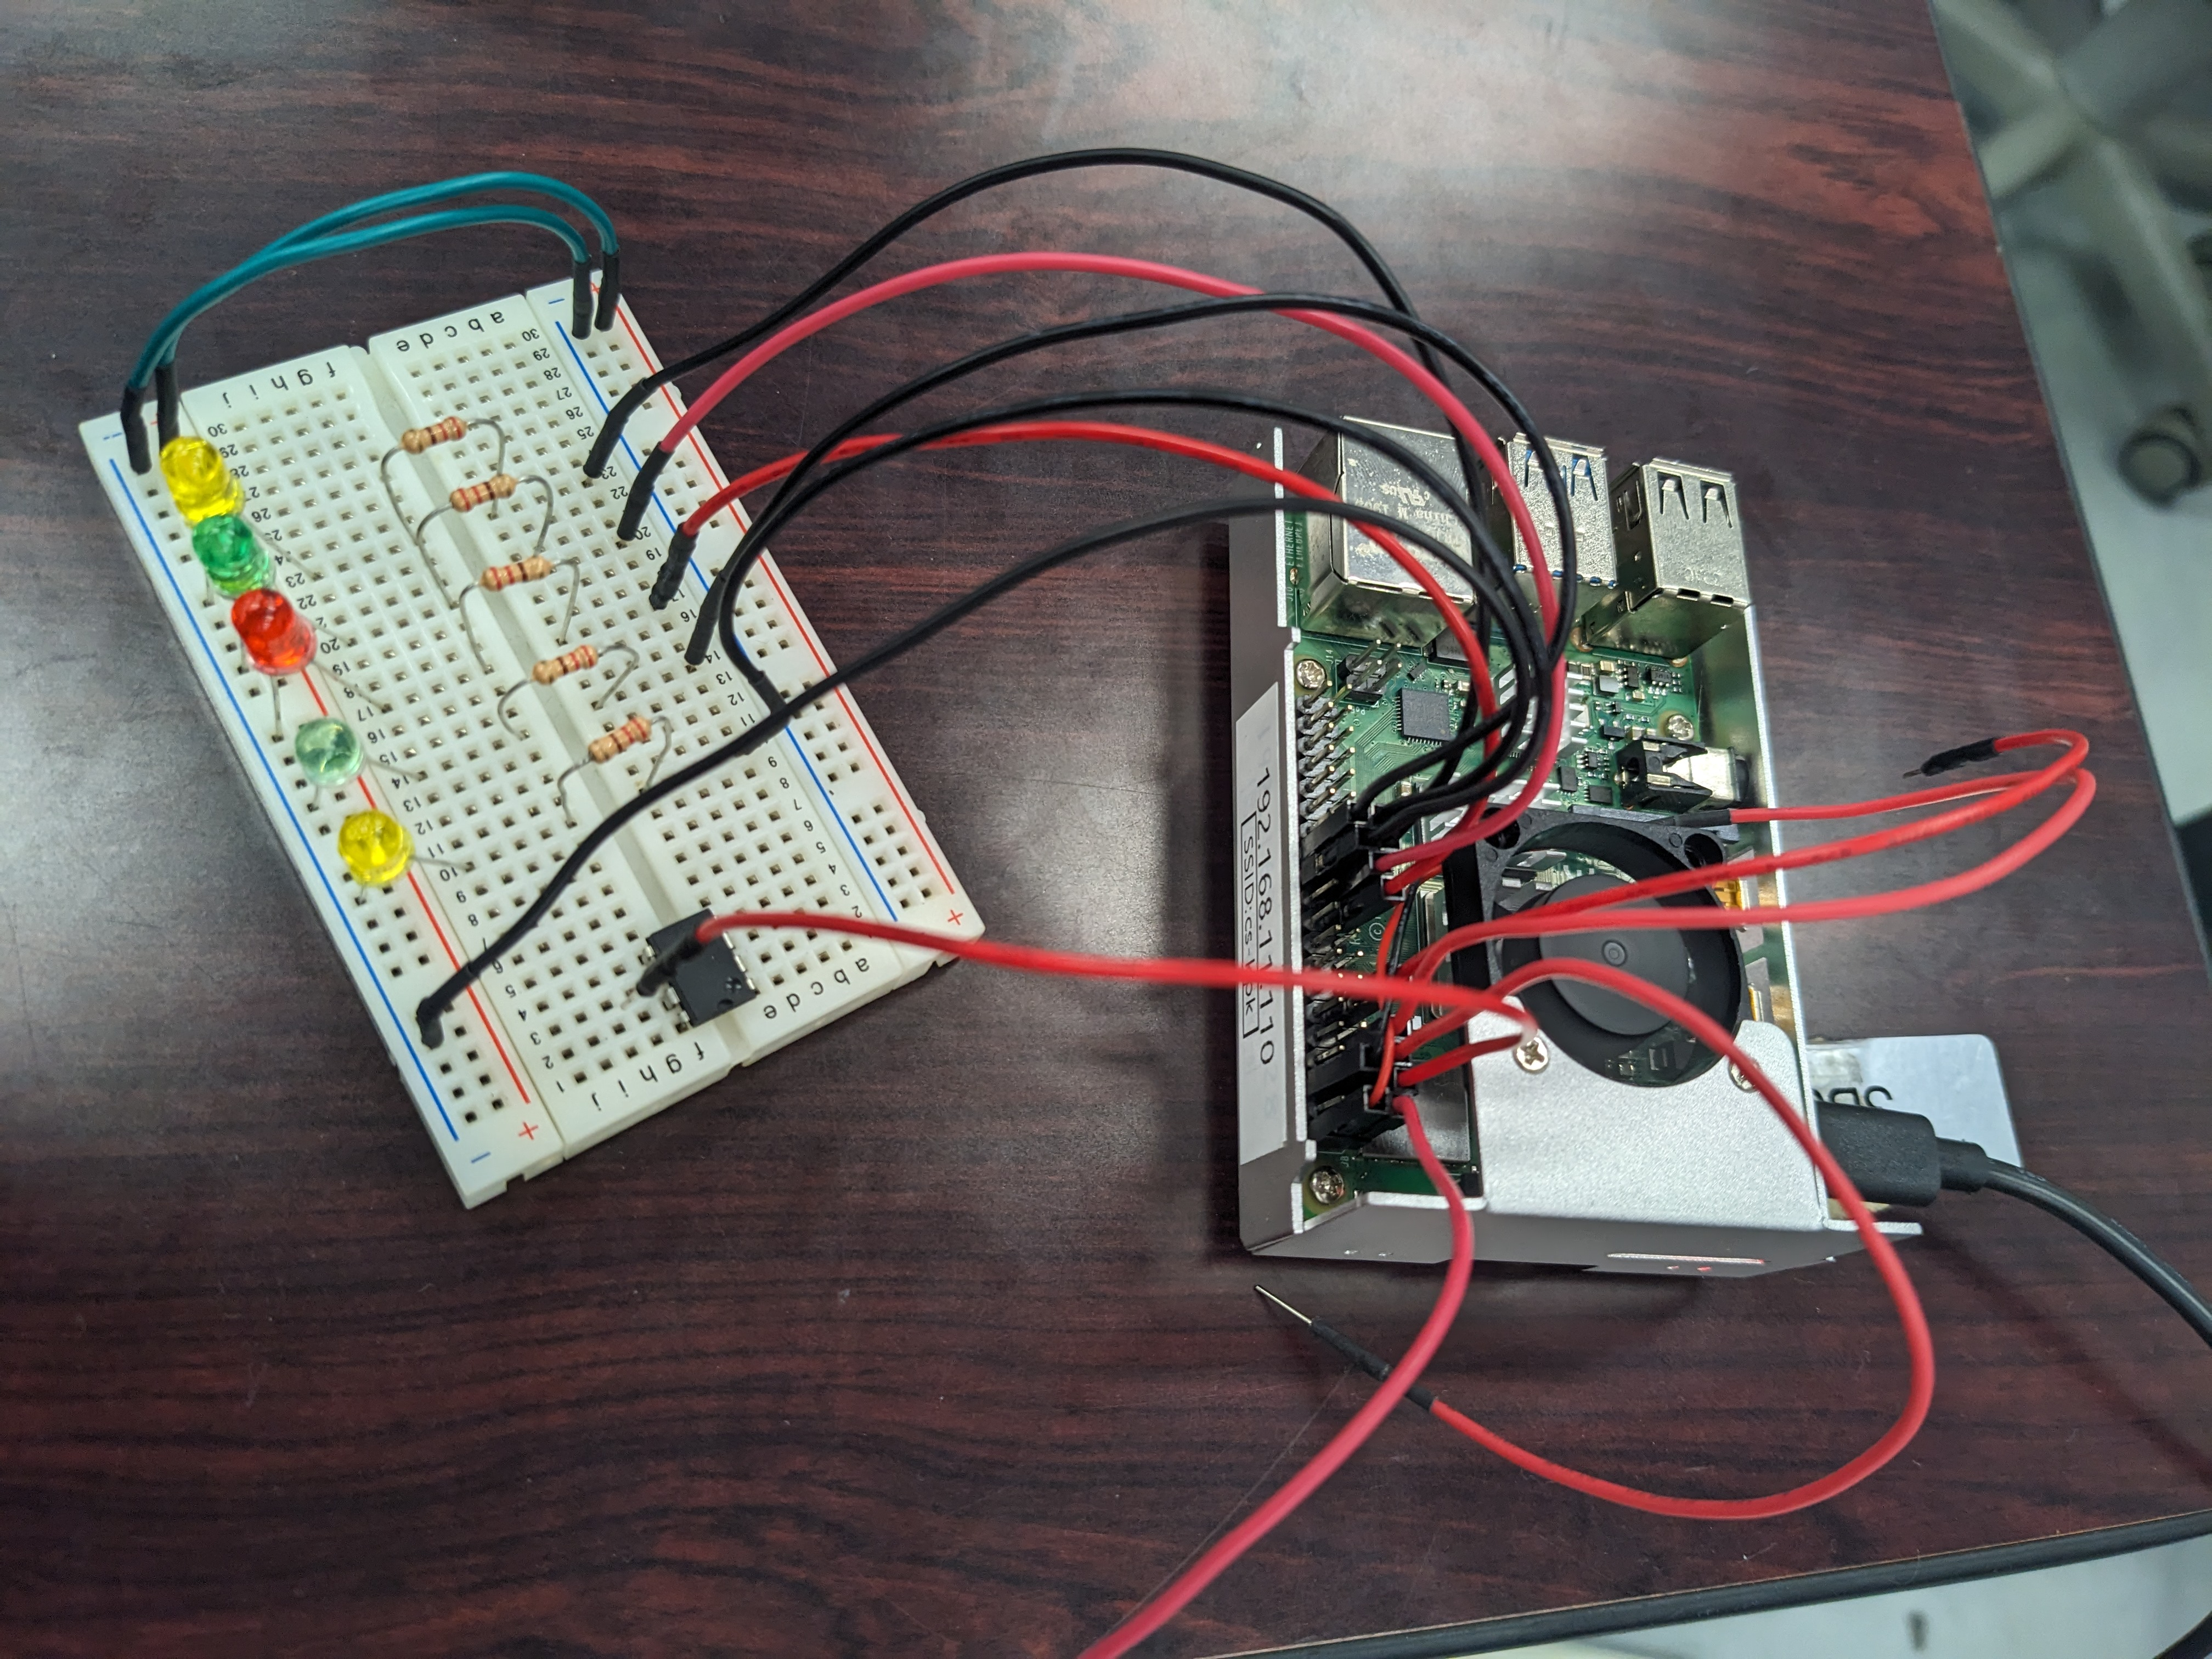
\includegraphics[width=0.5\textwidth]{materials/circuit_image.jpg}
\caption{Test setup showing the Raspberry Pi and LED configuration on the breadboard.}
\end{figure}

\subsection{Command Line Output}
The following screenshot shows the terminal output from a PC during the operation of the LED control system, demonstrating the successful reception and execution of commands to toggle the LEDs on and off.
Operation from a tablet was also executed and result shown to be successful.

\begin{figure}[h]
\centering
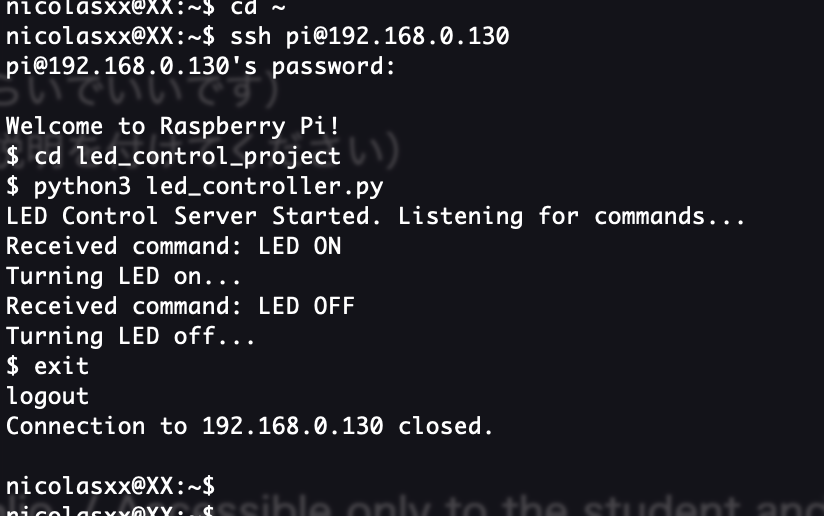
\includegraphics[width=0.5\textwidth]{materials/terminal_output.jpg}
\caption{Terminal output showing commands received and executed by the LED control system.}
\end{figure}

\section{Conclusion}
The project successfully demonstrates the use of a Raspberry Pi 4 and control control of LEDs over a network, in particular we propose the screenshot from the PC, highlighting the ease and flexibility of using standard components for IoT applications.
It is also highlighted that it is easy to control such a system using an android device.

\section*{References}
\begin{enumerate}
    \item \textbf{Mamanchuk N., University of Tsukuba}, Github, \today. Available online: \url{https://github.com/RIFLE}
\end{enumerate}

\end{document}
